\documentclass[11pt,a4paper]{article}
\usepackage[utf8]{inputenc}
\usepackage[T1]{fontenc}
\usepackage{amsfonts}
\usepackage[french]{babel}
\frenchbsetup{StandardLists=true} % à inclure si on utilise \usepackage[francais]{babel}
\usepackage{enumitem}
\usepackage{amssymb}
\usepackage{amsmath}
\usepackage[left=2cm,right=2cm,top=2cm,bottom=2cm]{geometry}
\usepackage{multirow}
\usepackage[dvipsnames]{xcolor}

\usepackage[T1]{fontenc}
\usepackage{fouriernc}
\usepackage{graphicx}

\usepackage{setspace}
\singlespacing

\usepackage{multicol}
\usepackage{caption}
\usepackage{fancyhdr}
\pagestyle{fancy}
\renewcommand\headrulewidth{1pt}
\fancyhead[L]{Lycée Denis Diderot }
\fancyhead[R]{Classe Terminale}
\setcounter{page}{6}\fancyfoot[C]{page \thepage}
\fancyfoot[R]{Année 2025 2026}
\fancyfoot[L]{Alexis RUIZ}
\usepackage{multirow,tabularx,booktabs}
\newcommand{\cadreblanc}[1]{%
\medskip\framebox[\linewidth][c]{%
\rule{0mm}{#1mm}}\par
\medskip}

\renewcommand{\arraystretch}{2}
\newcommand*\acocher{\quitvmode{\fboxsep0pt \fboxrule0.8pt \fbox{\vrule height1.8ex depth.1ex width0pt \vrule height0pt depth0pt width1.9ex }}}

\begin{document}
\center \LARGE{TP1 - Rôle de la diode}\
\\[0,3cm]

\normalsize

\hrule\
\\[0,2cm]

\flushleft \textbf{NOM :\\
Prénom:\\[0,2cm]
}
\hrule\
\\[0,2cm]

\fbox{MONTAGE 1} Réaliser le montage ci-dessous en utilisant les réglages suivants : \\
\begin{itemize}
\item tension alternative de 6 V;
\item au moins 2 périodes visualisables sur l'oscilloscope;
\item l'amplitude sur l'écran la plus grande possible.
\end{itemize}

\begin{center}

\includegraphics[scale=0.5]{images/circuit 1.png} 



\includegraphics[scale=0.25]{images/appel exam.png}\\   Appeler M Ruiz\\
\hrule\
\\[0,2cm]

Evaluation
\end{center}


\begin{center}
\renewcommand{\arraystretch}{2.8}
\begin{tabularx}{12 cm}{|c||X|}
\hline 

\hline
Composants présents sur la plaque & \\ 
\hline 
Les branchement de l'ocilloscope sont corrects  &  \\ 
\hline 
Le voltmètre délivre une tension alternative &  \\ 
\hline 
La tension est bien réglée sur 6 V  & \\ 
\hline 
Au moins deux périodes visualisables sur l'écran de l'oscillospe &  \\ 
\hline 
L'amplitude sur l'écran est bien la plus grande possible &  \\ 
\hline 

 
\end{tabularx}
\end{center}

\newpage

\fbox{Pré-requis} Rôle de la diode \\[2mm]

En classe de 5ième , vous avez découvert que la diode est un dipôle qui possède un sens passant et un sens bloquant. Retrouvez dans les circuits suivants les lampes qui sont allumées ou éteintes. 

\begin{center}
    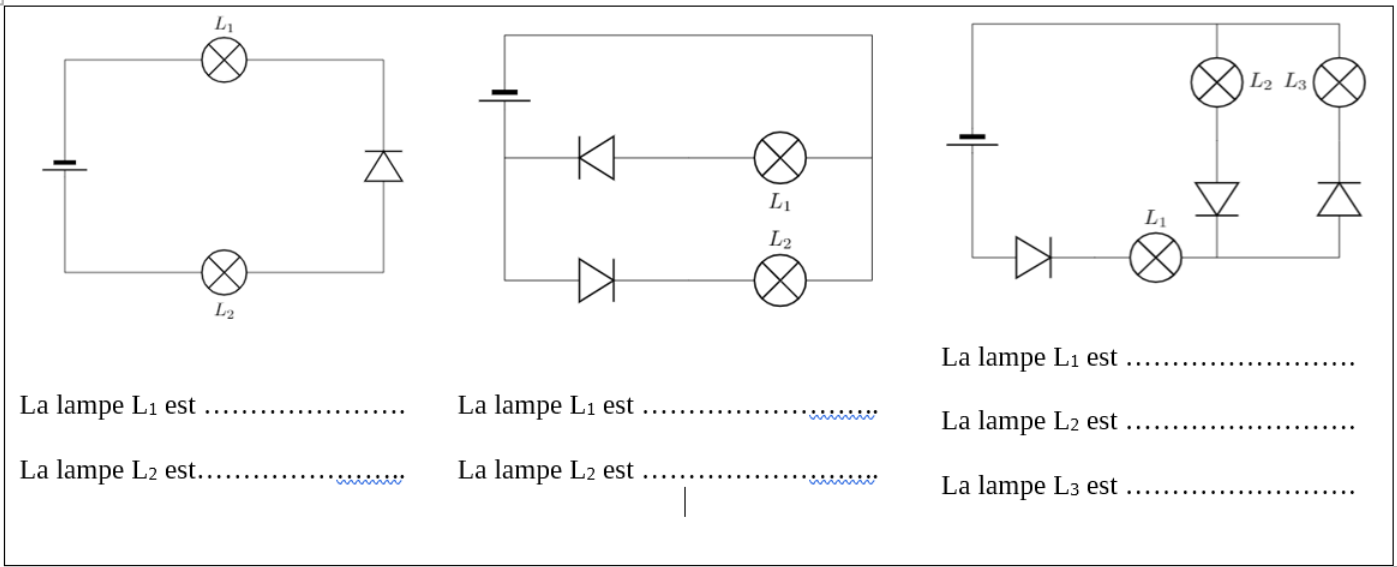
\includegraphics[scale=0.35]{images/prerequis.png}

\vfill 


\includegraphics[scale=0.5]{images/appel exam.png}\\   Appeler M Ruiz\\


\renewcommand{\arraystretch}{2.8}
\begin{tabularx}{6 cm}{|c||X|}
\hline
Evaluation &  \\
\hline 
\end{tabularx}
\end{center}

\vfill

\fbox{MONTAGE 2} Réaliser le montage ci-dessous en utilisant les réglages suivants : \\
\begin{itemize}
\item tension alternative de 6 V;
\item au moins 2 périodes visualisables sur l'oscilloscope;
\item l'amplitude sur l'écran la plus grande possible.
\end{itemize}

\begin{center}

\includegraphics[scale=0.25]{images/montage 1.png} 


\includegraphics[scale=0.5]{images/appel exam.png}\\   Appeler M Ruiz\\

\renewcommand{\arraystretch}{2.8}
\begin{tabularx}{12 cm}{|c||X|X|}
\hline
Évaluation & Montage & Réglages\\
\hline 


 
\end{tabularx}
\end{center}

\newpage

\begin{center}
Représenter l'oscillogramme obtenu à l'écran de l'oscilloscope.
\end{center}


\begin{multicols}{2}
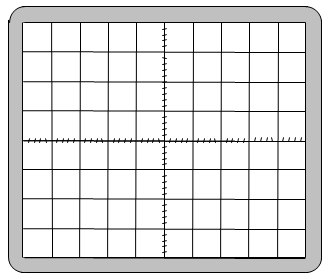
\includegraphics[scale=0.6]{images/ecran oscillo.png} 



\renewcommand{\arraystretch}{2.8}
\begin{tabularx}{8 cm}{|c||X|X|}
\hline
Valeurs & $U_{Max}=$ & $T=$\\
\hline 
\end{tabularx}

\renewcommand{\arraystretch}{2.8}
\begin{tabularx}{8 cm}{|c||X|X|}
\hline
Calculs & $U_{Eff}=$ & $f=$\\
\hline 
\end{tabularx}

\end{multicols}

La tension observée est-elle alternative ? Justifier votre réponse
\cadreblanc{20}

Quel est le rôle de la diode ? 
\cadreblanc{25}



\fbox{MONTAGE 3} Réaliser le montage ci-dessous en utilisant les réglages suivants : \\
\begin{itemize}
\item tension alternative de 6 V;
\item au moins 2 périodes visualisables sur l'oscilloscope;
\item l'amplitude sur l'écran la plus grande possible.
\end{itemize}

\begin{center}

\includegraphics[scale=0.25]{images/mpontage 3.png} 


\includegraphics[scale=0.5]{images/appel exam.png}\\   Appeler M Ruiz\\

\renewcommand{\arraystretch}{2.8}
\begin{tabularx}{12 cm}{|c||X|X|}
\hline
Évaluation & Montage & Réglages\\
\hline 
 
\end{tabularx}
\end{center}


\begin{multicols}{2}
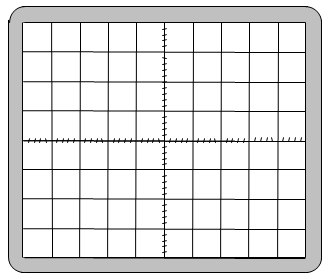
\includegraphics[scale=0.6]{images/ecran oscillo.png} 
Déterminer la valeur de la tension en V :\\
\cadreblanc {15}
De quel type de tension s'agit-il ? 
\cadreblanc{20}

\end{multicols}




Quel est le rôle du condensateur ? 
\cadreblanc{25}





\end{document}